\chapter{Discussions, conclusions and prospects}


 %The Belle II experiment is crucial in these channels because of the cleaner background environment and better sensitivity compared with LHCb.
\section{Discussions}
Based on the results and current status of the analysis, several important topics need to be discussed. In this section, we discuss the statistical and systematic uncertainty improvements in future based on the current results, as well as the importance of \textit{KsFinder} in this analysis. 
\subsection{Statistical uncertainty in future}
The precision on $\mathcal{S}$ requires the large luminosity of data as shown in Figure \ref{fig:sensitivity}, which includes both statistical and systematic uncertainties. With 50 ab$^{-1}$ luminosity from the full Belle II data sample in future, the statistical uncertainty is expected to be largely reduced. The $\it{CP}$ fit on the MC sample with different amount of events used reflects that the statistical uncertainty is reduced proportionally around factor of $\frac{1}{\sqrt{N}}$, where $N$ is the events used in $\it{CP}$ fit. Also,the wrong tag fraction is contributive to the statistical uncertainty. The performance of flavor tagging algorithm could be slightly improved in future. If so, the expected statistics of correctly tagged events could be increased. The reduced statistical uncertainty from this effect is considered to be marginal. Thus, the reduction of statistical uncertainty is assumed to mainly come from the increased data sample with current reconstruction efficiency, which is shown in Figure \ref{fig:stats_future}. At 50 ab$^{-1}$ luminosity, the statistical uncertainty is estimated to be $\sim 0.03$.

\begin{figure}[htpb]
	\centering
	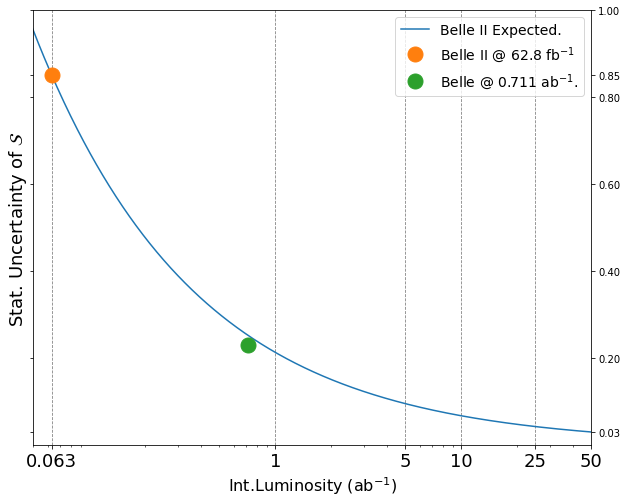
\includegraphics[width=0.7\linewidth]{stats_b2}
	\caption{Statistical uncertainty of $\mathcal{S}$ extrapolation based on the current result of $B^0 \to K_S^0  K_S^0  K_S^0$ in Belle II, where the orange is the current value and the green is the Belle result at 0.711 ab$^{-1}$ $\Upsilon$(4S) data.}
	\label{fig:stats_future}
\end{figure}

From Table \ref{tab:b0stats}, the current $B^0$ reconstruction efficiency is 34\% which could be further optimized mainly by improving $K_S^0$ reconstruction efficiency. As discussed in Section 3, the reconstruction efficiency and vertexing quality become worse for long-flight $K_S^0$ particles. This is mainly due to the limitation of CDC-only tracking and the hit filters on the SVD layers. The current Belle II track finding algorithm rises a requirement for SVD hits that at least two or more SVD hits have to be associated from a same track so that they can be used together to form a track. If a $K_S^0$ decays outside of layer 5 at 10.4 cm, even though the daughter tracks could pass the SVD layer 6, they are much likely to become two CDC-only tracks unless they pass the overlapped regions at the edges of SVD layers. 

This effect is shown in Figure \ref{fig:svd-r-xx}, where \textit{SVD00} type $K_S^0$ starts to appear at SVD layer 5 instead of layer 6. The requirement of the SVD hits in the current tracking algorithm is needed to suppress the beam background and SVD noise strips that create a large fraction of random single hits. Thus, the actual sensitive volume of SVD is reduced and the $K_S^0$ reconstruction efficiency is negatively affected. 
In future, the improvement of our tracking algorithm is expected to remove this requirement while still be able to effectively reduce single-hit background. The fraction of the \textit{SVD00} type $K_S^0$ will be reduced to provide a better vertexing quality as well.

In general, the expected $B^0$ signal yield can be improved in future and help to further reduce the statistical uncertainty. From Figure \ref{fig:stats_future}, the extrapolated statistical uncertainty at $0.711$ ab$^{-1}$ is comparable with the Belle result. 
When the integrated luminosity reaches about 9 ab$^{-1}$, the statistical uncertainty is reduced to $\sim 0.072$ which is equivalent to the current systematic uncertainty. At 50 ab$^{-1}$ integrated luminosity, the major contribution will be systematic uncertainty if no improvement is assumed. We take the extrapolated statistical uncertainty of $\sim 0.030$ at 50 ab$^{-1}$ as a conservative value for estimating the total uncertainty later.



\begin{figure}[htpb]
	\centering
	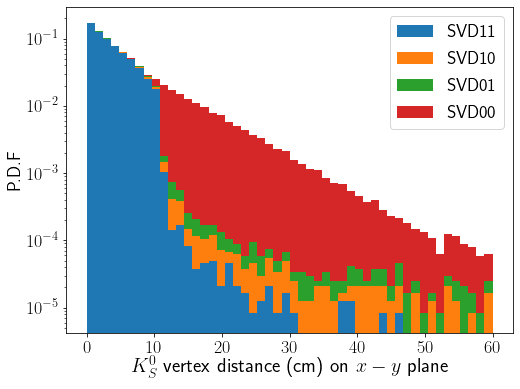
\includegraphics[width=0.7\linewidth]{ks-r-svdxx}
	\caption{The $K_S^0$ are categorized into 4 types. \textit{SVD11} (\textit{SVD00}) are the ones whose daughter pion tracks have non-zero (zero) SVD hits. \textit{SVD10} (\textit{SVD01}) stands for the ones whose only positive (negative) charged pion track contains SVD hits.
		 The distribution is the $K_S^0$ flight length on $x-y$ plane for each category of $K_S^0$, where \textit{SVD00} type $K_S^0$ start to appear at about SVD layer 5.}
	\label{fig:svd-r-xx}
\end{figure}

\subsection{Systematic uncertainty in future}
\begin{comment}
As discussed in the section 1, the NP effects that potentially contributes to the $B^0\to \phi K_S^0$ could also affect $B^0 \to K_S^0  K_S^0  K_S^0$. In the current SM correction, the QCD factorization (QCDF) scan approach suggests the expected upper-limit for $\Delta \mathcal{S}$ is about 0.05~\cite{b2book}. 
\end{comment}

When the statistical uncertainty is largely reduced to a comparable level with the systematic uncertainty in future, it is important to evaluate the reducible and irreducible systematic uncertainties in $B^0 \to K_S^0  K_S^0  K_S^0$ for future data collection based on the current measurement result. If no improvement on systematic uncertainty is expected from the current evaluation, it is still challenging to validate the evidence of the NP effects against the small theoretical predictions with the full Belle II luminosity in future.
%QCDF generally predicts definite or preferred signs of the $\Delta \mathcal{S}$ shift, which implies a definite pattern of shifts to be compared with data\cite{b2book}. At present thereis no significant tension between these predictions and data. 

The reducible systematic sources mainly benefit from the increased luminosity of the experiment data or the larger production of the MC samples, depending on how the corresponding parameters are determined.
The  systematic uncertainties from signal $\Delta t$ shape and the fit bias will be reduced possibly by the increased MC sample, including both \textit{signal MC} and \textit{generic MC}. The systematic uncertainties from signal fraction, background $\Delta t$ shape and wrong tag fraction will be reduced by the larger luminosity of data in future. 
As an initial study in early operation with very low statistics, it is assumed that these reducible sources are achieved by the increased number of events where the reduced uncertainties are scaled by the fraction of squared-root of increased events. To the contrary, the irreducible sources mainly refer to the ones that are not improved with increased data luminosity or MC samples, such as the irreducible vertexing related sources and tag-side interference~\cite{b2book}.

For the signal $\Delta t$ shape parameters related to $\it{CP}$-side resolution function, the improvement could also come from the better VXD performance and improved tracking algorithm.
In the Belle II original prospects, the new PXD detector would be contributive to reduce about 50\% of the systematic uncertainties caused by the vertexing resolution. This assumption is made by referencing the evaluation using $J/\psi K^0$ channel in Ref.~\cite{b2book} compared to the Belle result. Current, the vertexing resolution on the $\it{CP}$-side from our analysis is close to that of the Belle. However, such vertex-related improvement might be hard to fully achieved due to the lack of the direct tracks from the IP in our analysis, which makes the vertexing improvement less promising. 
In the mean time, the uncertainties of $\it{CP}$-side resolution parameters can be reduced if more \textit{signal MC} samples are used. This is dependent on the actual MC production plan, where even the signal yield from the current 1 million \textit{signal MC} is already much more than the signal events in 50 ab$^{-1}$ data. Considering both the unclear improvements from the vertexing quality and the future MC, we keep the reduction factor of 2 as the expected value in 50 ab$^{-1}$ data. The current contribution from $\it{CP}$-side resolution parameters is $\sim 0.030$, which can be reduced to $0.015$ based on this assumption. On the other hand, if the improvement from the vertexing quality is very small and the mount of \textit{signal MC} is not changed as a conservative case, we assume the $\it{CP}$-side systematic uncertainty is the same value as the current one.

For the tag-side parameters, the current contribution is $\sim 0.016$ determined from the MC control sample corresponding to 2 ab$^{-1}$ luminosity. Unlike the $\it{CP}$-side, tag-side vertex reconstruction is almost universal for the different decay modes. We only expect that the reduced systematic uncertainties from these parameters come from the same mount of MC control sample as 50 ab$^{-1}$, which is going to be $\sim 0.003$. To be conservative, the vertexing improvement for the tag-side is not assumed because we do not perform the full reconstruction of $B$ mesons. 

In Table  \ref{tab:sig_shape}, the improvement where both $\it{CP}$- and tag-sides uncertainties are reduced is calculated to be $0.015$ while a conservative case that only tag-side is improved is also considered, which is $\sim0.030$.
\begin{table}[H]
		\centering
		\caption{ Signal $\Delta t$ shape systematic uncertainties of $\mathcal{S}$ expected at 50 ab$^{-1}$. The second and third columns are the expected reduced systematic uncertainties for both $\it{CP}$/tag-side improvements or only tag-side improvement.}
		\label{tab:sig_shape}
		\begin{tabular}{c| c| c }
			\hline
			Luminosity (50 ab$^{-1}$) & both ($\it{CP}$/tag) improved & only tag-side improved \\
			\hline
			signal $\Delta t$ shape &  $\sim0.015$ & $\sim0.030$\\
			\hline
		\end{tabular}
\end{table}
For the signal fraction contribution which is the largest source at this moment, it mainly suffers from the very low statistics in data that causes the inaccurate modeling of signal shape parameters. Therefore the uncertainties of signal fraction parameters are expected to be reduced quickly with the increased experiment data in future. To be noted, the uncertainties from signal fraction parameters are not directly included in the $\it{CP}$ fit model. The 2D signal extraction model is changed every time the parameters are floated and $f^{sig}$ is updated for $\it{CP}$ fit. We compare the systematic uncertainty obtained from \textit{generic MC} with the Belle result and the luminosity scaled Belle II result.
 Using 1 ab$^{-1}$ \textit{generic MC}, the combined contribution on $\mathcal{S}$ uncertainty by floating $\pm 1 \sigma$ for each parameter is calculated to be $\sim 0.013$. This estimation is close to the observed systematic uncertainty in the Belle data which is  $\sim0.015$~\cite{kang2020measurement} and the Belle II data scaled value $\sim 0.011$. The luminosity scaling factor $1/\sqrt{N}$ still works well in this case. So we assume this source can be reduced to $\sim 0.0016$ by factor $\sqrt{50/0.063}$ as shown in Table \ref{tab:sig_f} in 50 ab$^{-1}$ Belle II data.

\begin{table}[htpb]
	\centering
	\caption{ Signal fraction systematic uncertainties of $\mathcal{S}$ expected at 50 ab$^{-1}$.}
	\label{tab:sig_f}
	\begin{tabular}{c| c}
		\hline
		Luminosity (50 ab$^{-1}$) & Improved uncertainty \\
		\hline
		Signal fraction &  $\sim0.0016$ \\
		\hline
	\end{tabular}
\end{table}

For the background $\Delta t$ shape, the systematic uncertainties comes from the parameters determined by the sideband data. Thus, the systematic uncertainty is reduced by factor $\sqrt{50/0.063}$ to be $\sim 0.001$ as listed in Table \ref{tab:bkg_shape}.

\begin{table}[htpb]
	\centering
	\caption{ Background $\Delta t$ shape systematic uncertainties of $\mathcal{S}$ expected at 50 ab$^{-1}$.}
	\label{tab:bkg_shape}
	\begin{tabular}{c| c}
		\hline
		Luminosity (50 ab$^{-1}$) & Improved uncertainty \\
		\hline
		Background $\Delta t$ shape &  $\sim0.0014$ \\
		\hline
	\end{tabular}
\end{table}

For the contributions of wrong tag fraction, the uncertainties of $w$ in each $r$-bin is expected to be reduced with more tagging control samples. The current wrong tag fraction is taken from 8.7 fb$^{-1}$ early Belle II data~\cite{abudinen2020first}. The expected uncertainties at 50 ab$^{-1}$ Belle II data is close to zero as listed in Table \ref{tab:wtag_50ab}, regarded as a negligible source.

\begin{table}[htpb]
	\centering
	\caption{ Wrong tag fraction systematic uncertainties of $\mathcal{S}$ expected at 50 ab$^{-1}$.}
	\label{tab:wtag_50ab}
	\begin{tabular}{c| c}
		\hline
		Luminosity (50 ab$^{-1}$) & Improved uncertainty \\
		\hline
		wrong tag fraction &  $\sim0.00049$\\
		\hline
	\end{tabular}
\end{table}

For the fit bias contribution, currently the values are taken by the statistical fit error using 300000 events in \textit{signal MC}. If MC sample used in future could be at least 100 times more than one million, then the fit error is possible to be smaller than input-output difference. From the current MC production plan of the Belle II, the  \textit{signal MC} sample recommended by MC production group is typically in a range of several millions. So the foreseen systematic uncertainty is still going to be the fit error, where we take a 50\% reduction of the value $\sim0.0098$ from Tabel \ref{tab:fitbias} as an estimation, listed in Table \ref{tab:fitbias_full}.
\begin{table}[htpb]
	\centering
	\caption{ Fit bias systematic uncertainties of $\mathcal{S}$ expected at 50 ab$^{-1}$.}
	\label{tab:fitbias_full}
	\begin{tabular}{c| c}
		\hline
		Luminosity (50 ab$^{-1}$) & Improved uncertainty \\
		\hline
		fit bias &  $\sim 0.005$ \\
		\hline
	\end{tabular}
\end{table}

Concluded from the above discussion, the reducible systematic uncertainties by using increased MC and data in the full Belle II luminosity are estimated and summarized in Table \ref{tab:reducedsys}. It is clear that the dominated contribution in future Belle II data for systematic uncertainty is the $\it{CP}$ side resolution, indicating the finer study on $\it{CP}$ side resolution model for no IP-originated tracks is important.

The impact of using \textit{KsFinder} receives contribution from the data-MC mismatch, which can be be improved by a better data-MC consistency. For physics parameters $\Delta m_d$ and $\tau_{B^0}$, the uncertainties could be reduced by the improved physics input. The vertex reconstruction options are not contributing much in this analysis mostly because they are partially reflected by the signal $\Delta t$ shape contributions. Using proper IP constraint and tighter vertex cuts, the signal $\Delta t$ shape will contribute less and vertex reconstruction could contribute more in future. The tag-side interference contribution is referenced to be $\sim0.001$ as a small source from the Belle study~\cite{yosuke2011measurement}.   The current estimations from \textit{KsFinder} ($\sim0.004$), physics parameters ($\sim$0.007), the vertex reconstruction ($\sim$0.019) and tag-side interference($\sim0.001$) are assumed to be unchanged in the 50 ab$^{-1}$ Belle II luminosity to have a conservative expectation on $\mathcal{S}$ systematic uncertainty, shown in Table \ref{tab:unchangedsys}. 

It is worth noting that these estimations on the future systematic uncertainties are very preliminary. Some assumptions and expectations are subject to change in future. The vertexing quality and IP conditions can not be precisely assessed at this moment, so as the potential improvements from them. The models used in the signal extraction, resolution functions and $\it{CP}$ fit could be modified in future based on the new observations from data and MC, which might contain the different sources of systematic uncertainties. The misalignment of the VXD is not studied at the current stage, but should be included as one of the systematic uncertainty if it is found to be not negligible in future. Overall, we keep these estimations rather conservative to be a baseline for the future studies.
 
\begin{table}[htpb]
	\centering
	\caption{ Improved systematic uncertainties of $\mathcal{S}$ expected at 50 ab$^{-1}$. The value in the parenthesis stands for the case that only tag-side resolution is improved and no improvement on $\it{CP}$ side resolution is implemented. }
	\label{tab:reducedsys}
	\begin{tabular}{c| c}
		\hline
		Sources & Improved uncertainty (50 ab$^{-1}$) \\
		\hline
		signal $\Delta t$ shape &  $\sim$0.015($\sim$0.030)\\
		Signal fraction &  $\sim$0.002 \\
		Background $\Delta t$ shape &  $\sim0.001$\\
		wrong tag fraction &  $\sim0.000$\\
		fit bias &  $\sim0.005$\\
		\hline
		Total & $\sim$0.016 (0.030)\\
		\hline
	\end{tabular}
\end{table}

\begin{table}[htpb]
	\centering
	\caption{The unchanged systematic uncertainties at 50 ab$^{-1}$ based on the current luminosity of the Belle II data.}
	\label{tab:unchangedsys}
	\begin{tabular}{c| c}
		\hline
		Sources & Unchanged uncertainty (50 ab$^{-1}$) \\
		\hline
		\textit{KsFinder} & $\sim$0.004\\
		physics parameters &  $\sim$0.007 \\
		vertex reconstruction &  $\sim$0.019\\
		tag-side interference &  $\sim0.001$\\
		\hline
		Total & $\sim$0.021\\
		\hline
	\end{tabular}
\end{table}

\subsection{Total uncertainty of $\Delta \mathcal{S}$ at 50 ab$^{-1}$}
The total systematic uncertainty of $\mathcal{S}$ in the 50 ab$^{-1}$ Belle II luminosity is estimated based on the improved sources from Table \ref{tab:reducedsys} and the unchanged sources from Table \ref{tab:unchangedsys}. If $\it{CP}$ side resolution is not improved, the systematic uncertainty is $\sim$0.037. If the $\it{CP}$ side resolution functions is 50\% improved, the systematic uncertainty is reduced to  $\sim0.026$. Both are shown in Table \ref{tab:sys_full}.
\begin{table}[htpb]
	\centering
	\caption{The systematic uncertainty expected in 50 ab$^{-1}$ Belle II luminosity. The first column is the current value of systematic uncertainty of $\mathcal{S}$ in $B^0 \to K_S^0  K_S^0  K_S^0$. The second and third columns are the systematic uncertainties for both $\it{CP}$/tag-side improvements or only tag-side improvement used in the combined estimation.}
	\label{tab:sys_full}
	\begin{tabular}{c| c | c |c}
		\hline
		Luminosity(ab$^{-1}$) & current~(0.0628) & $\it{CP}$/tag~(50)& only-tag~(50)\\
		\hline
		Syst.Uncert. on $\mathcal{S}$ & $0.072$ & $\sim$0.026 & $\sim0.037$\\
		\hline
	\end{tabular}
\end{table}


By adding in quadrature using estimated statistical and systematic uncertainties, the total uncertainty for $\mathcal{S}$ in $B^0 \to K_S^0  K_S^0  K_S^0$ in 50 ab$^{-1}$ Belle II luminosity is estimated, as shown in Table \ref{tab:err_full}. Total uncertainty of $\sim 0.048$ or $\sim 0.040$ is expected depending on if the $\it{CP}$-side resolution is improved or not. Considering that the total uncertainty from $B^0\to J/\psi K_S^0$ at that time is expected to be $\sim 0.005$~\cite{b2book}, $\Delta S$ sensitivity  will be dominated by the total uncertainty in $B^0 \to K_S^0  K_S^0  K_S^0$. The current Belle result from $B^0 \to K_S^0  K_S^0  K_S^0$ on $\Delta S$ is $0.71-0.67\sim0.04$ without taking into account any uncertainty. Considering the total uncertainty from the current Belle result is about 0.24, the center value of $\mathcal{S}$ is still quite likely to be 5$\sigma$ away from that of $J/\psi K^0_S$ under a future uncertainty at $0.040\sim 0.048$.
In general, a total uncertainty at about $0.040\sim 0.048$ for $\Delta S$ at Belle II full luminosity is expected to be a much better probe for addressing whether the NP effects in $B^0 \to K_S^0  K_S^0  K_S^0$ exist. 

\begin{table}[htpb]
	\centering
	\caption{The total uncertainty of $\mathcal{S}$ in $B^0 \to K_S^0  K_S^0  K_S^0$ expected in 50 ab$^{-1}$ Belle II luminosity, calculated from the expected statistical and systematic uncertainties. The second and third columns are the total uncertainties for both $\it{CP}$/tag-side improvements or only tag-side improvement used in the combined estimation.}
	\label{tab:err_full}
	\begin{tabular}{c|c|c |c}
		\hline
		Luminosity (ab$^{-1}$) & current~(0.0628)&$\it{CP}$/tag~(50) & only-tag~(50)\\
		\hline
		Tot.Ucert. on $\mathcal{S}$ & $0.853$ & $\sim0.040$ & $\sim0.048$ \\
		\hline
	\end{tabular}
\end{table}

\subsection{\textit{KsFinder} importance}
While monitoring the uncertainties of the $\it{CP}$ parameters is crucial in searching the hidden NP effects, avoiding wrongly estimated $\it{CP}$ asymmetry in the measurement is also critical. If a total uncertainty at $\sim 0.03$ is achieved in future, however, the center value of $\mathcal{S}_{3K_S^0}$ is wrongly shifted away from $\mathcal{S}_{J/\psi K_S^0}$, it can lead to a very wrong conclusion about the discovery of the NP effects.
The \textit{KsFinder} contributes to improve the signal purity for measuring $\it{CP}$ parameters, which is essential in controlling the potential effect introduced by the large fraction of background events that yield random $\it{CP}$ asymmetry due to the statistical fluctuation.
The signal extraction and $\it{CP}$ fit on the 1 ab$^{-1}$ \textit{generic MC} sample without \textit{KsFinder} are performed. In this case, we remove the \textit{KsFinder} cut in Table \ref{tab:b0select} and apply the cut $cosVertexMomentum > 0.9$ which can only achieve $\sim 82\%$ purity for $K_S^0$ in \textit{signal MC}. The signal fraction in the signal region defined by $M_{bc}$ and $\Delta E$ is considerately lower than that with using \textit{KsFinder}. The stacked histograms of $M_{bc}$ and $\Delta E$ with much higer background are shown in Figure \ref{fig:hist_2D_highBG} where the red component is signal. There are 352 true signal events and 543 background events inside the signal region by count. In the meanwhile, the 2D fit on $M_{bc}$ and $\Delta E$ are shown in Figure \ref{fig:2Ddata_noks}. From the 2D fit, the signal events number is $389\pm19$ and background events number is $502\pm15$. The comparison of the number of events obtained by different methods is summarized in Table \ref{tab:ksbias}.
\begin{table}[htpb]
	\centering
	\caption{The number of the signal and background events using \textit{KsFinder} or cut on \textit{cosVertexMomentum} are obtained by the 2D fit, which are compared with the numbers by directly counting the events with $isSignal=1 (0)$.
	It is clear that the number of events obtained by using \textit{KsFinder} is closer to the MC truth.}
	\label{tab:ksbias}
	\begin{tabular}{c| c |c}
		\hline
		Selection & signal  & background \\
		\hline
		${FBDT\_Ks>0.74}$ (fit) & $341\pm20$ & $61\pm17$ \\
		${FBDT\_Ks>0.74}$ (MC) & 336 & 68\\
		${cosVertexMomentum>0.9}$ (fit) & $389\pm19$ & $502\pm15$\\
		${cosVertexMomentum>0.9}$ (MC) & 352 & 543\\
		\hline
	\end{tabular}
\end{table}

From Table \ref{tab:ksbias}, by using \textit{KsFinder}, the true average signal fraction in signal region from 1 ab$^{-1}$ \textit{generic MC} is 83.2\%, and the fit result is $(84.8\pm3.7)\%$. To contrary, by only using ${cosVertexMomentum>0.9}$, the true average signal fraction is 39.3\% and the fit result is $(43.7\pm1.4)\%$. In future when the instantaneous luminosity of the SuperKEKB ramps up to a much higher level, the fraction of fake $K_S^0$ could also rise, too. The signal extraction on a high background event collection might be hard to obtain the signal fraction correctly.
Therefore, the development of \textit{KsFinder} is particularly important in the precise $\it{CP}$ measurement for $B^0 \to K_S^0  K_S^0  K_S^0$ by providing high purity signal events. The current performance of \textit{KsFinder} is presenting a purity about 95\% in $K_S^0$ reconstruction which means there is still a margin for the improvements. The targeted purity and background rejection power of \textit{KsFinder} in future is $\sim 99\%$ on average. The data/MC consistency should also be improved so the current correction ratio $R_{B^0}$ is expected to be reduced to $\sim 1.00\pm 0.01$. Thus the systematic uncertainty from different \textit{KsFinder} responses in between data and MC is assumed to be $\mathcal{O}(0.001)$ as a negligible contribution. 



\begin{figure}[htbp]
	\begin{minipage}[b]{0.5\linewidth}
		\centering 
		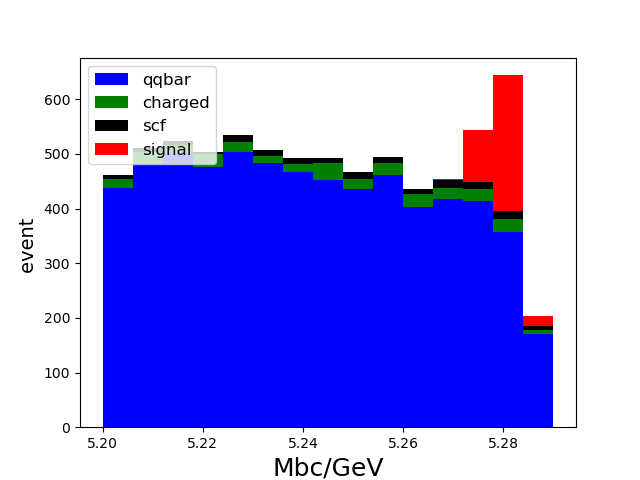
\includegraphics[height=6cm]{figures/hist_stacked_generic_mbc_noksfinder.png}
		\label{}
	\end{minipage}
	\begin{minipage}[b]{0.5\linewidth}
		\centering 
		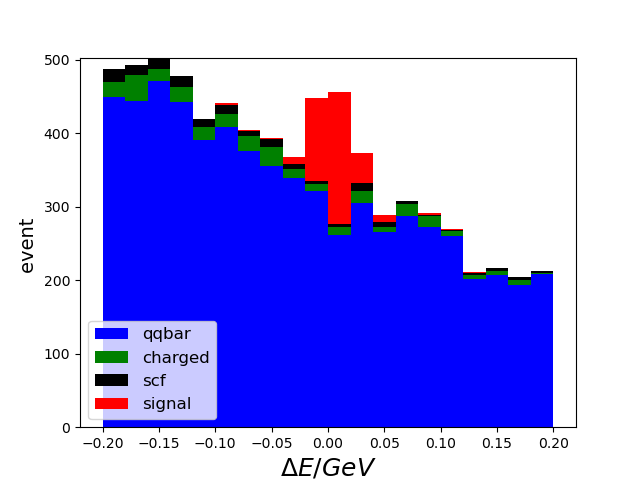
\includegraphics[height=6cm]{figures/hist_stacked_generic_dE_noksfinder.png}
		\label{}
	\end{minipage}
	\caption{$M_{bc}$ and $\Delta E$ stacked histogram of  1 ab$^{-1}$ \textit{generic MC} sample replacing $FBDT\_Ks>0.74$ by ${cosVertexMomentum}>0.9$ in Table \ref{tab:b0select} as a selection criteria, showing a much worse signal significance.}
	\label{fig:hist_2D_highBG}
\end{figure}





\begin{figure}[htbp]
	\begin{minipage}[b]{0.5\linewidth}
		\centering 
		\includegraphics[height=6cm]{figures/ds_gen_mbc_2D}
		\label{}
	\end{minipage}
	\begin{minipage}[b]{0.5\linewidth}
		\centering 
		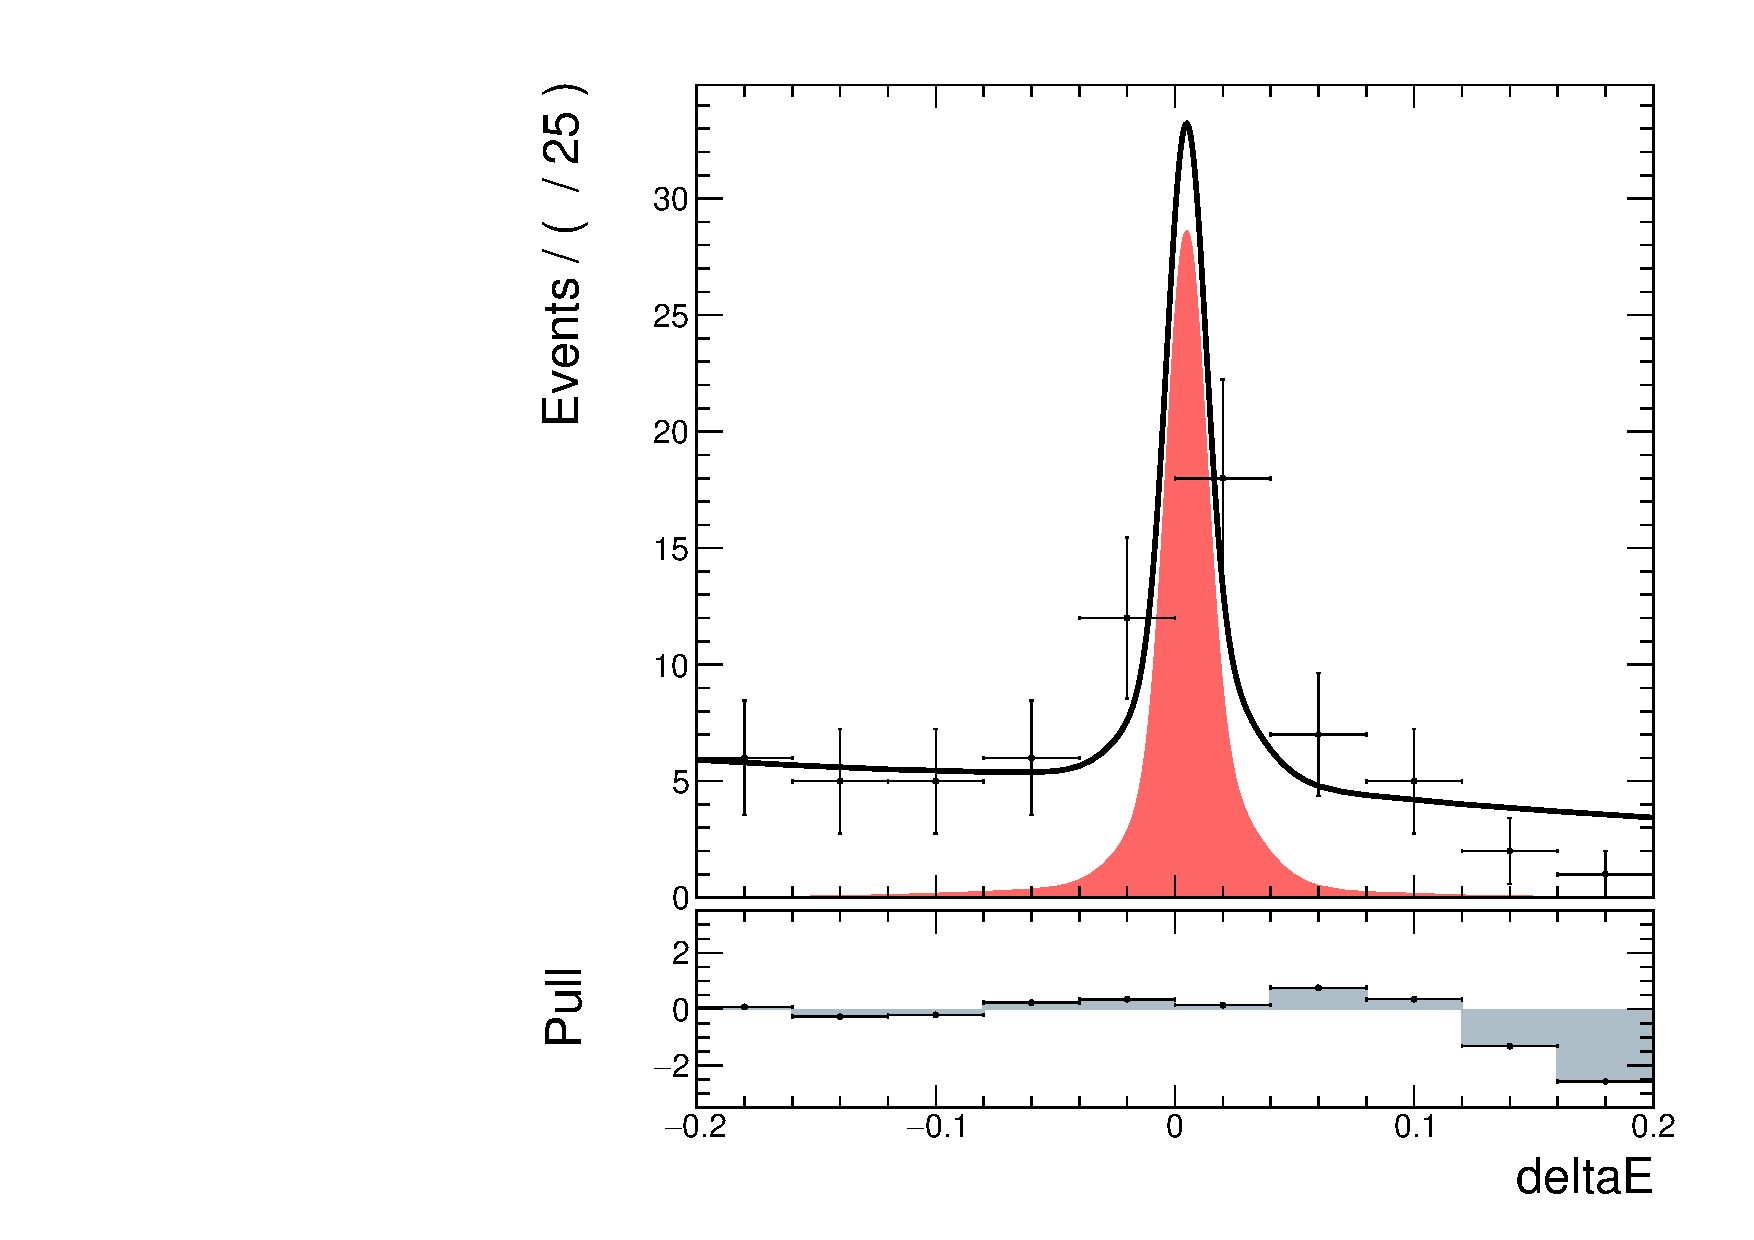
\includegraphics[height=6cm]{figures/ds_gen_deltaE_2D}
		\label{}
	\end{minipage}
	\caption{$M_{bc}$ and $\Delta E$ 2D fit on 1 ab$^{-1}$ \textit{generic MC} sample, replacing $FBDT\_Ks>0.74$ by ${cosVertexMomentum}>0.9$ in Table \ref{tab:b0select}. The red is signal component.}
	\label{fig:2Ddata_noks}
\end{figure}

\section{Conclusions}
In this thesis, we perform the analysis of the $\it{CP}$ parameter measurement in $B^0 \to K_S^0  K_S^0  K_S^0$ using the early Belle II data, which is targeted to search for the NP effects in the penguin dominated $b\to s$ transition. The reconstruction of $K_S^0$ is initially done by using a traditional cut-based method with a large fraction of fake candidates. Thus a new MVA-based \textit{KsFinder} is developed by using FastBDT algorithm  which can effectively improve the signal purity. For the reconstruction of $B^0$, we take advantage of two variable $M_{bc}$ and $\Delta E$ to select the events with a sufficient continuum background suppression. To obtain the signal fraction for each $B^0$ events, a 2D fit model is established and fitted using 62.8 fb$^{-1}$ data. 
The model of the resolution of vertex positions has been studied using MC sample and sideband data based on the understanding of vertex reconstruction performance in the current Belle II detectors. To make a proper use of the reconstructed vertex information and perform a $\it{CP}$ fit compactly, a new $\it{CP}$ fitter is built and being validated, which will serve as a multi-functional analysis tool for the Belle II $\it{CP}$ violation study in future. 
The $\it{CP}$ parameter measurement is performed based on the validation of analysis strategies by the blind analysis that shows a consistent result for $\it{CP}$ parameters compared to the simulation input. The linearity and pull of the $\it{CP}$ fit are checked to demonstrate the reliability of the fit procedures. The fit result on $B^0$ lifetime using the experiment data is also agreed with the current value in PDG with a relatively large statistical uncertainty due to the low statistics of data.

After the $\it{CP}$ fit procedures are validated, the $\it{CP}$ parameters $\mathcal{S}$ and $\mathcal{A}$ using 62.8 ab$^{-1}$ Belle II early data in 2019 and 2020 spring and summer are obtained. The result is

\begin{equation}\label{eq:data_fit_cp}
\begin{split}
\mathcal{S}=- \text{sin}(2\phi_1) & = -0.82 \pm 0.85~(\text{stat}) \pm 0.07~(\text{syst})~, \\
\mathcal{A} & = -0.21\pm 0.28~(\text{stat}) \pm 0.06~(\text{syst})~.\\
\end{split}
\end{equation}  

The result agrees with the prediction of the Standard Model and the previous results from Belle~\cite{kang2020measurement} and BaBar~\cite{Lees:2011nf}. The measurement precision of $\it{CP}$ parameters in this thesis is majorly limited by the large statistical uncertainty.


\section{Prospects}
Even though the current result on $\it{CP}$ parameters are dominated by the large uncertainty, the previous discussions about the future results have shown a good potential of searching for the NP effects in $B^0 \to K_S^0  K_S^0  K_S^0$ based on the current analysis in this thesis. At integral luminosity at 50 ab$^{-1}$, the uncertainty on $\mathcal{S}$ would be reduced to a comparable value around $0.040\sim0.048$ realistically, as shown in Figure \ref{fig:tot_exp}{\protect\footnotemark}, where the statistical and reducible systematic uncertainties are assumed to be scaled by the squared root of the integrated luminosity. The expected sensitivity in full Belle II data is proven to be competitive and the analysis workflow is built which will be further improved along with the future Belle II data taking and MC production. The progress that has been made in this thesis paves a well-constructed and solid path for searching the NP effects in time dependent $\it{CP}$ violation study of $B^0 \to K_S^0  K_S^0  K_S^0$ at the full Belle II luminosity in future.
 
\begin{figure}[htpb]
	\centering
	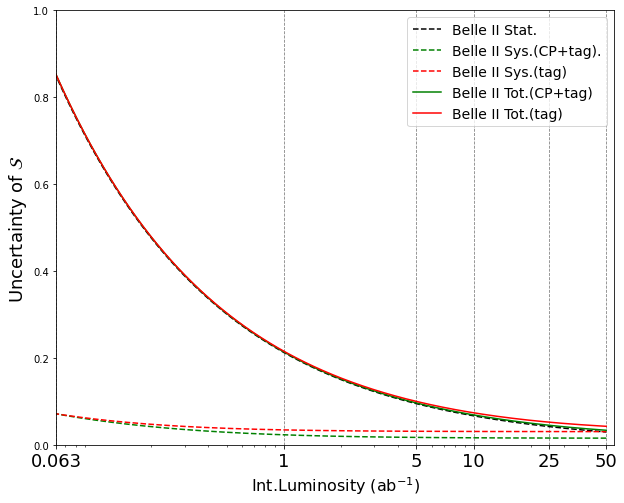
\includegraphics[width=0.7\linewidth]{tot_unc_1}
	\hspace*{1.5cm}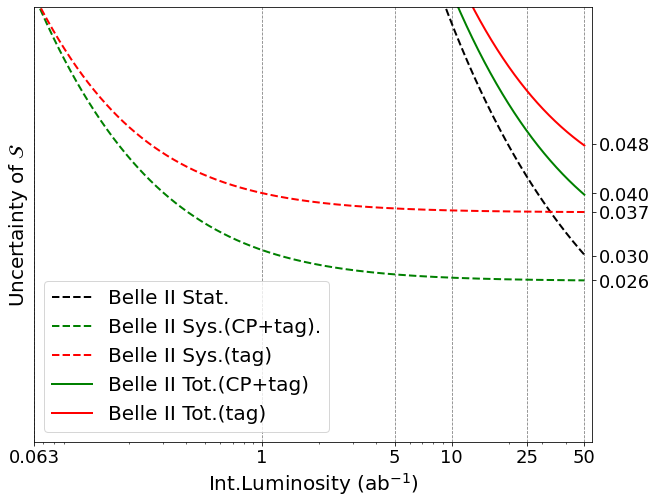
\includegraphics[width=0.7\linewidth]{tot_unc_2}
	\caption{The expected total uncertainty of $\mathcal{S}$ in $B^0 \to K_S^0  K_S^0  K_S^0$, where the dashed lines are the statistical (black), $\it{CP}$/tag-side improved systematic (green) and only tag-side improved systematic (red) uncertainties, with the corresponding solid lines as the total uncertainties. The top is the overview for the whole Belle II luminosity range from now, and the bottom is $y$-axis zoom-in. }
	\label{fig:tot_exp}
\end{figure}
\footnotetext{For the continuous extrapolation of the systematic uncertainties, an assumption is used that the reducible part is approximately scaled by the square-root of the future luminosity and the irreducible part is treated as a constant. Thus two Equations are formed:  $0.072^2=a/0.0628+b$ and $0.026^2~(0.037^2) =a/50+b $ where $a$ and $b$ present the reducible and irreducible part, which are used as the coefficients of the extrapolating function.}
